\documentclass[12pt]{report}

\title{Topic modeling bla bla}

\renewcommand{\thesection}{\arabic{section}}

\setcounter{secnumdepth}{5}
\setcounter{tocdepth}{5}

\usepackage{amsfonts}
\usepackage{graphicx}
\usepackage{cite}
\usepackage{algorithm2e}


\begin{document}

\maketitle
\tableofcontents


\begin{abstract}
This is a simple paragraph at the beginning of the document. 
A brief introduction about the main subject.
\end{abstract}


\section{Introduction}
This is where you tell people why they should bother reading your article.


\section{Theoretic background}

In this chapter we will present some basic theoretic background about topic
modeling. To deal with extensive text body, machine learning researchers have
developed topic modeling: a suite of methods that analyze the words of the
original text to discover the themes that run through the data and detect
hidden semantic structures by analyzing a corpus. By marking up the documents
using these topics and by using the resulting structure, the model can be used
for organization, finding similar documents, or any other similar tasks. A
topic is here defined as a probability distribution of words, meaning that
certain words are more likely within a certain topic. Since the topics emerge
from the analysis of the original texts, topic modeling algorithms do not
require any prior annotations or labeling of the documents.

In order to apply a topic model to our data, the first question we must answer
is how to represent documents. For understanding of natural language one must
obviously preserve the order of the words in documents. However, for many
large-scale data mining tasks, it is sufficient to use a simple representation
that loses all information about word order. Given a collection of documents,
the first task to perform is to identify the set of all words used at least
once in at least one document. This set is called the vocabulary. Often, we
reduce the size of the vocabulary by keeping only words that are used in at
least a small percentage of the documents. Words that are found only once are
often misspellings or other mistakes. Although the vocabulary is a set, we fix
an arbitrary ordering for it so we can refer to word 1 through word $m$ where
$m$ is the size of the vocabulary. Once the vocabulary has been fixed, each
document is represented as a vector with integer entries of length $m$. If this
vector is $x$ then its $j$-th component $x_j$ is the number of appearances of
word $j$ in the document. The length of the document is $n=\sum\limits_{j=1}^m
x^j$.

Many applications of if topic modeling also eliminate from the vocabulary so-
called “stop” words. These are words that are common in most documents and do
not correspond to any particular subject matter. They include pronouns (you,
he, it), connectives (and, because, however), prepositions (to, of, before),
and auxiliaries (have, been, can, should). Stop words may also include generic
nouns (amount, part, nothing) and verbs (do, have). A collection of documents
is represented as a two-dimensional matrix where each row describes a document
and each column corresponds to a word. Each entry in this matrix is an integer
count; most entries are zero. It makes sense to view each column as a feature.

Some further common concepts and terms in topic modeling:

- A word is defined as an item from a vocabulary indexed from ${1, ..., V}$,
where V is the size of the vocabulary. All words are represented as unit-basis
vectors with one component equal to one and the rest equal to zero.

- A document is a collection of words denoted by $w = {w_1, ..., w_N}$, where
$w_n$ is the $n$th word and $N$ is the total number of words in the collection.

- A corpus is a collection of documents in a dataset. It is denoted $D = {w_1,
..., w_M}$, where $w_m$ is the $m$th document in the corpus and $M$ is the
total number of documents.

- Latent variables are variables that may not be directly observed, unlike
observable variables. Latent variables can instead be inferred from other
observable variables.

- Polysemy is the capacity for a word to have multiple related meanings. An
example of this is the word “plant” which can mean a living organism of the
kind exemplified by trees, herbs etc., or a place where an industrial or
manufacturing process takes place.

- Synonymy is the capacity for several words to have similar meanings such as
the words “buy” and “purchase”.

\subsection{The Multinomial Distribution}

Once we have a representation for individual documents, the natural next step
is to select a model for a set of documents. It is important to understand the
difference between a representation and a model. A representation is a way of
encoding an entity as a data structure. A model is an abstraction of a set of
entities, for example a probability distribution. Given a training set of
documents, we will choose values for the parameters of a probabilistic model
that make the training documents have high probability. Then, given a test
document, we can evaluate its probability according to the model. The higher
this probability is, the more similar the test document is to the training set.


The probability distribution that we use is the multinomial. Mathematically,
this distribution is:

\begin{equation}
p(x;\theta) = \left(\frac{n!}{\prod\limits_{j=1}^m x^j!}\right)\left
(\prod\limits_{j=1}^m \theta_j^{x_j}\right)
\end{equation}

where the data $x$ are a vector of non-negative integers and the parameters
$\theta$ are a real-valued vector. Both vectors have the same length $m$.
Intuitively, $\theta_j$ is the probability of word $j$ while $x_j$ is the count
of word $j$. Each time word $j$ appears in the document it contributes an amount
$\theta_j$ to the total probability, hence the term $\theta_j^{x_j}$. The
components of $\theta$ are non-negative and have unit $\sum\limits_{j=1}^m
\theta_j = 1$. A vector with these properties is called a unit vector.

Like any discrete distribution, a multinomial has to sum to one, where the sum
is over all possible data points. Here, a data point is a document containing
$n$ words.


\subsection{Basic models in topic modeling}

First, we’ll introduce some basic models for topic modeling. The Latent Semantic
Indexing, or LSI, was presented by Deerwester et al. in 1990. The model manages
to deal with the problem that multiple terms can refer to the same meaning,
i.e. synonymy. However, it is not as successful regarding polysemy. The reason
is that every term is represented as just one point in the so-called latent
semantic space. Furthermore, a word that can mean two or more different things
is represented as a weighted average of the different meanings.
 
After LSI was introduced, Hofmann presented the Probabilistic Latent Semantic
Indexing, or PLSI model. PLSI is a so-called topic model where each word in a
document is generated from a single “topic” which results in that each document
in a corpus can be represented with a topic distribution. Later, in 2003 Blei et
al. presented the Latent Dirichlet Allocation, or LDA. As opposed to PLSI, LDA
is a statistically generative model for documents where each word in a document
can be generated by all topics.

\subsubsection{Latent Semantic Indexing (LSI)}

Latent Semantic Indexing was one of the earliest methods for finding
relationships between documents and the words that occur in them. In LSI a
term-document matrix is created by analyzing the corpus, where the rows
correspond to words and columns to documents. Each element in this sparse
matrix describes the number of times a word occurs in a document but this term
count can also be weighted with for instance TF-IDF. Letting each word
represent a dimension in a very high dimensional space, a document can be seen
as a vector with components corresponding to its weighted term counts.

A low-rank approximation of the term-document matrix is created using Single
Value Decomposition, SVD, which creates new dimensions, called concepts, as
linear combinations of the original words. This allows similarity measures and
clustering methods by reducing the volume of the word space and thus making
this space more densely populated.


The drawbacks with LSI are mainly the lack of a statistical foundation in the
model. LSI is based on linear algebra instead of probabilistic modeling leaving
it with a small toolbox for what can be achieved using the model.
	

\subsubsection{Probabilistic Latent Semantic Indexing (PLSI)}


Probabilistic Latent Semantic Indexing evolved from LSI and uses the same
concept of finding a lower rank approximation of the term-document occurrence
matrix. The difference is that instead of being based on linear algebra, PLSI
is based on a mixture decomposition using a latent class model. PLSI associates
an unobserved class variable $z$ with each document-word observation pair $(w,
w)$. This $z$ can be seen as a topic, since it is a probability distribution
over words. As a generative model, PLSI can be defined in the following way for
a corpus $D$:

\begin{enumerate}
\item Pick a document $w$ with probability $p(w)$
\item For each of the $N$ words in $w$:
\begin{description}
\item (a) Pick a topic $z$ with probability $p(z|w)$
\end{description}
\begin{description}
\item (b) Generate a word $w$ with probability $p(w|z)$
\end{description}
\end{enumerate}


The result from PLSI is that every document is represented as mixing proportions
for the topics, given by $p(z|w)$. Even though PLSI is generative for the
analyzed corpus, it is not generative for new documents, which means is that
there is no clear way of assigning probability to a document that is not part
of the training data. Another problem is that the number of parameters in the
model grows linearly with the number of documents.


\subsubsection{Latent Dirichlet Allocation (LDA)}

LDA is a topic model that was first presented as a graphical model for topic
discovery by David Blei, Andrew Ng, and Michael I. Jordan in 2003. The basic
idea is that documents exhibit multiple topics. LDA is a generative statistical
model that allows sets of observations to be explained by unobserved groups
that explain why some parts of the data are similar. For example, if
observations are words collected into documents, it posits that each document
is a mixture of a small number of topics and that each word's occurrence is
attributable to one of the document's topics. This is similar to PLSI, except
that in LDA the topic distribution is assumed to have a Dirichlet prior (see
2.3.3.1). In practice, this results in more reasonable mixtures of topics in a
document. The reduced document description result in PLSI is a vector where
each element describes the mixing proportion for a topic. A limitation with
PLSI is that there is no generative model for these proportions, making it
difficult to handle unseen documents. The Latent Dirichlet Allocation model
tries to solve this limitation by setting a Dirichlet prior on the topic
distribution.
 
Suppose that we have a collection of documents, and we want to find an
organization for these, i.e. we want to do unsupervised learning. A common way
to do unsupervised learning is to assume that the data were generated by some
probabilistic process, and then to infer the parameters of this process. The
generative process is a specification of a parametrized family of
distributions. Learning is based on the principle of maximum likelihood, or
some refinement of this principle such as maximum a posterior probability.
 
The basic idea in LDA is that we define a topic to be a Dirichlet distribution
over a fixed vocabulary. Technically, the model assumes that the topics are
generated first, before the documents. Now for each document in the collection,
we generate the words in a two-stage process:


\begin{enumerate}
\item Randomly choose a distribution over topics.
\item For each word in the document:
\begin{description}
	\item (a) Randomly choose a topic from the distribution over topics in step 1.
\end{description}
\begin{description}
	\item (b) Randomly choose a word from the corresponding distribution over the 
	vocabulary.
\end{description}
\end{enumerate}


This statistical model reflects the intuition that documents exhibit multiple
topics. Each document exhibits the topics with different proportion (step 1);
each word in each document is drawn from one of the topics (step 2b), where the
selected topic is chosen from the per-document distribution over topics (step
2a). All the documents in the corpus share the same set of topics, but each
document exhibits those topics with different proportion - that’s the
distinguishing characteristic of LDA. A more detailed explanation of the model
follows in section 2.3.3.2.


\paragraph{Dirichlet distribution}


The Dirichlet distribution is a way to model random probability mass functions
(PMFs)\footnote{If you roll 1000 dice, the theoretical odds of any particular
number showing up (i.e. a 1, 2, 3, 4, 5, or 6) are 1/6. However, you won’t get
that exact distribution in a real experiment due to manufacturing defects. If
you have ten dice, each die will have its own probability mass function (PMF).}
for finite sets. It is also sometimes used as a prior in Bayesian statistics.
The Dirichlet is the multivariate generalization of the beta distribution. It
is an extension of the beta distribution for modeling probabilities for two or
more events; when the result of the event has only 2 values, the Dirichlet
distribution is equal to the beta distribution.


The Dirichlet distribution is a prior for the multinomial distribution. This
means that if the prior distribution of the multinomial parameters is Dirichlet
then the posterior distribution is also a Dirichlet distribution (with
parameters different from those of the prior).

The Dirichlet process is a way to model randomness of a probability mass
function (PMF) with unlimited options (e.g. an unlimited amount of dice in a
bag). The process is similar Polya’s Urn, only instead of having a set number
of ball colors you have an unlimited amount:

\begin{itemize}
\item Start out with an empty urn.
\item Randomly pick a colored ball and place it in the urn.
\item Then choose one option:
\begin{enumerate}
\item Randomly pick a colored ball and place it in the urn.
\item Randomly remove a colored ball from the urn, then put it back with another 
ball of the same color.
\end{enumerate}
\end{itemize}
 
As the number of balls in the urn increase, the probability of picking a new
color decreases. The proportion of balls in the urn after an infinite amount of
draws is a Dirichlet process.


\paragraph{Model}

LDA is a probabilistic model of text documents, which assumes a collection of 
K topics. Each topic defines a multinomial distribution over the vocabulary 
and is assumed to have been drawn from a Dirichlet 
$\beta_k \sim Dirichlet(\eta)$. 

In LDA, each document is represented by a mixture of the topics, with weight
$\theta_w^2$ for topic $z$ in document $w$. These weight have a Dirichlet prior,
parameterized by a hyper-parameter $\alpha$. Each topic is a probability
distribution over the vocabulary, with probability $\beta^w_z$ for word $w$ in
topic $z$.
 
For each document $w$, in corpus $D$, the LDA generative process is as follows:

\begin{enumerate}
	\item Draw topic distribution $\theta_w \sim Dir(\alpha)$
	\item For each of the $N$ words $w_n$:
	\begin{description}
	\item (a) Draw a specific topic $z_n \sim Multinomial(\theta)$
	\item (b) Draw a word $w_n \sim Multinomial(\beta_{zn})$
	\end{description}
\end{enumerate}


As seen in step 1, each document contains topics in different proportions,
determined by the scaling parameter $\alpha$. The individual words are drawn
from one of the $k$ topics in step (b), where the probability of each word
within a topic is parameterized by a $k \times V$ matrix , where $V$ is the
size of the specified vocabulary. The most probable words in each topic could
be used to identify the topic and gives an intuitive description for the topic.

We can analyze a corpus of documents with LDA by examining the posterior
distribution of topics $\beta$, topic proportions $\theta$ and topic
assignments $z$ conditioned on the documents. This reveals latent structure in
the collection that can be used for prediction or data exploration. This
posterior can't be computed directly; it is usually approximated using Markov
Chain Monte Carlo (MCMC) or variational inference. Both methods are effective,
but also present significant computational challenges in large data sets
~\cite{onlineLDAvb}. In our implementation, we're using the online variational
LDA model, which is described in section 2.2.3.4.
 
The key difference in LDA compared to PLSI is that the process outlined above
actually is generative for documents. This means that, given a new document,
one can use the parameters learned previously to estimate the topic
distribution $\theta$ for this new document.
 
A limitation with the standard LDA model is the fix vocabulary. This means that
new words cannot enter the model and that you have to know a priori what words
will model the corpus effectively. A setting where this could be problematic is
when analyzing twitter data where new words in the form of slang, names and
hashtags emerge over time. Another limitation is the fact that one has to state
the number of topics the model should use. This is not a big issue, but could
lead to some of the resulting topics to be insignificant.

\begin{figure}
\centering
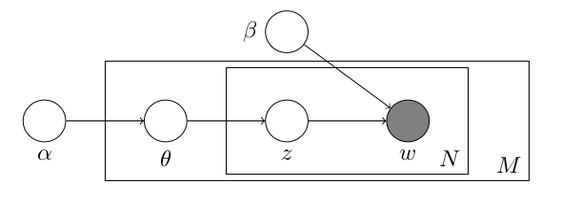
\includegraphics[width=0.6\textwidth]{LDA_standard_model.png}
\caption{Plate notation of the standard LDA model}
\end{figure}


\paragraph{Expectation Maximization}

The Expectation Maximization, or EM, algorithm is an approach to deriving an
algorithm for approximately obtaining maximum likelihood of variables in a
statistical model. Normally one obtains a maximum likelihood solution by taking
partial derivatives of the likelihood function with respect to all variables,
setting these derivatives to zero and solving the equations simultaneously.

Due to latent variables it is not always possible to solve the equations
directly and instead one typically gets two sets of equations that depend on
each other. The EM algorithm uses the idea that one could choose starting
values for the latent variables in the first set of equations, use the result
in the second set of equations, and then alternate between the two sets until
convergence.

Consider a statistical model accompanied by a set of observed data $X$, a set of
latent data $Z$, a set of latent variables $\theta$ and a likelihood function
$L(\theta \mid X, Z)$. The marginal likelihood of the observed data is then

\begin{equation}
L(\theta \mid X) = p(X \mid \theta) = \sum\limits_{Z} p(X, Z \mid \theta)
\end{equation}

which determines the maximum likelihood estimate of the latent variables. The
sum is however often intractable and the EM algorithm solves this problem by
iterating the following two steps:

\begin{itemize}
\item \textbf{Expectation step (E - step)}: For the current estimate of the 
parameters $\theta^t$, calculate the expected value of the log likelihood function:
\begin{equation}
Q(\theta \mid \theta^t) \leftarrow \mathbb{E}_{Z \mid X, \theta^t}
 [\log(L(\theta \mid X, Z))]
\end{equation}
\item \textbf{Maximization step (M - step)} Maximize the expected value function 
with regard to the parameters:
\begin{equation}
\theta^{t + 1} \leftarrow arg \max\limits_{\theta} Q(\theta \mid \theta^t)
\end{equation}
\end{itemize}

\paragraph{Variational Inference}

Learning the various distributions (the set of topics, their associated word
probabilities, the topic of each word, and the particular topic mixture of each
document) is a problem of Bayesian inference. In the original paper it's being
used a variational Bayes approximation of the posterior distribution;
~\cite{blei2003latent} alternative inference techniques use Gibbs sampling and
expectation propagation. The goal of variational inference is to approximate an
intractable probability distribution $p$, with a tractable one $q$, in a way
that makes them as close as possible given a similarity measure. In this thesis,
variational inference is used to approximate the posterior distribution of
latent variables. A new distribution over the hidden variables $q(z, \beta)$
(called the variational distribution) is  introduced. This new distribution has
properties such that it can be efficiently computed. 

The variational distribution is a function of a set of free parameters that are optimized such that the variational distribution is as close as possible to the 
actual target posterior distribution where closeness is measured in terms of KL divergence.
Minimizing the KL divergence between the variational distribution and the target
posterior is equivalent to maximizing the Evidence Lower BOund (ELBO) which is

\begin{equation}
L(q) = E_q [log p(x, z, \beta)] -  E_q [log q(z, \beta)]  
\end{equation}

The variational distribution has the property that it can be efficiently
computed. This is done by making each hidden variable independent of each other.

\begin{equation}
q(z, \beta) = q(\beta \mid \lambda) \prod\limits_{n=1}^N \prod\limits_{j=1}^J q(z_{nj} \mid \phi_{nj})   
\end{equation}

The posterior over the per-word topic assignments $z$ is parameterized by
$\phi$, the posterior over per-document topic weights $\theta$ is parameterized
by $\gamma$, and the posterior over the topics $\beta$ is parameterized by
$\lambda$. Furthermore, each hidden variable is governed by its own variational
parameter so the variational parameters $\lambda$ governs the global variables
$\beta$ and the variational parameters $\phi_n$ govern the local variables $z_n
q(\beta \mid \lambda)$ and $q(z_{nj} \mid \phi_{nj})$ take the same form as the
complete conditionals $p(\beta \mid x, z, \alpha)$ and $p(z_{nj} \mid x_n, z_{n,
-j}, \beta)$, but the natural parameters are now $\lambda$ and $\phi_{nj}$,
respectively to give

\begin{equation}
q(\beta \mid \lambda) = h(\beta) exp(\lambda^T t(\beta) - \alpha_g(\lambda))
\end{equation}
\begin{equation}
q(z_{nj} \mid \phi_{nj}) = h(z_{nj}) exp(\phi_{nj}^T t(z_{nj}) - \alpha_l(\phi_{nj}))
\end{equation}

Where $h(.)$ is called the base measure, $\alpha(.)$ is called the log-
normalizer, $\eta(.)$ is called the natural parameter, and $t(.)$ is called the
sufficient statistics. Furthermore, we also assume that the prior distribution
over $\beta$ is part of the exponential family. We maximize the ELBO objective
function with a coordinate ascent procedure. We find its gradient with respect
to the global variational parameter $\lambda$ and find the value of $\lambda$
that sets the gradient to zero. We do the same thing for the local parameters
$\phi_n$. We iterate between these updates until we converge to the maximum of
the ELBO. The updates are given without proof, but the general procedure is to
write the ELBO in terms of parameter of interest (either $\lambda$ or $\phi_n$)
then take the gradient and set it to zero.

\begin{equation}
\lambda = E_q[\eta_g(x, z, \alpha)]
\end{equation}
\begin{equation}
\phi_{nj} = E_q[\eta_l(x_n, z{n, -j}, \beta)]
\end{equation}

Therefore the updates of each variational parameter are equal to the expected
value of the natural parameters of the complete conditionals. A simple outline 
of the algorithm ~\cite{alexminnar} is given below


\begin{algorithm}[H] 
\SetAlgoLined

Initialize $\lambda^{(0)}$ randomly.
\Repeat{the ELBO converges}{
	\For{each local variational parameter $\phi_{nj}$}{\label{forins}
		Update $\phi_{nj}^{(t)} = \mathbb{E}_{q^{(t - 1)}}[\eta_{l,j}(x_n, z_{n,-j}, \beta)]$.
	}
	Update the global variational parameters, $\lambda^{(t)} = \mathbb{E}_{q^{(t)}}[\eta_g (z_{1:N}, x_{1:N})]$.
}
\caption{Variational Bayes for LDA} 
\end{algorithm}


As you can see, in the local parameter update (in the $for$ loop), we have to
iterate over every data point in the data set which is computationally
expensive. The algorithm above has constant memory requirements and empirically
converges faster than collapsed Gibbs sampling. However, it still requires a
full pass through the entire corpus in each iteration. It can be slow to apply
to very large datasets. An online variational inference algorithm is proposed by
Hoffman et all. ~\cite{onlineLDAvb} for fitting $\lambda$, the parameters to the
variational posterior over the topic distributions $\beta$. The "online LDA" is
nearly as simple as the variational algorithm, but converges much faster for
large datasets.

\section{Related work}

\section{Methodology}

\section{Analysis and results}

\section{Conclusion}

\section{Future work}

\bibliography{references}{}
\bibliographystyle{plain}

\end{document}